% !TEX TS-program = pdflatex
% !TEX encoding = UTF-8 Unicode

% This is a simple template for a LaTeX document using the "article" class.
% See "book", "report", "letter" for other types of document.

\documentclass[11pt]{article} % use larger type; default would be 10pt

\usepackage[utf8]{inputenc} % set input encoding (not needed with XeLaTeX)

%%% Examples of Article customizations
% These packages are optional, depending whether you want the features they provide.
% See the LaTeX Companion or other references for full information.

%%% PAGE DIMENSIONS
\usepackage{geometry} % to change the page dimensions
\geometry{a4paper} % or letterpaper (US) or a5paper or....
% \geometry{margins=2in} % for example, change the margins to 2 inches all round
% \geometry{landscape} % set up the page for landscape
%   read geometry.pdf for detailed page layout information

%%% Line Spacing
\usepackage{setspace}
\onehalfspacing

\usepackage{graphicx} % support the \includegraphics command and options

% \usepackage[parfill]{parskip} % Activate to begin paragraphs with an empty line rather than an indent

%%% PACKAGES
\usepackage{booktabs} % for much better looking tables
\usepackage{array} % for better arrays (eg matrices) in maths
\usepackage{verbatim} % adds environment for commenting out blocks of text & for better verbatim
\usepackage{subfig} % make it possible to include more than one captioned figure/table in a single float
\usepackage{amsmath, amssymb, amsthm, lastpage}
% These packages are all incorporated in the memoir class to one degree or another...

%%% HEADERS & FOOTERS
\usepackage{fancyhdr} % This should be set AFTER setting up the page geometry
\pagestyle{fancy} % options: empty , plain , fancy
\renewcommand{\headrulewidth}{0pt} % customise the layout...
\lhead{Team \# 16677}\chead{}\rhead{Page \thepage\ of \pageref{LastPage}}
\lfoot{}\cfoot{\thepage}\rfoot{}

%%% SECTION TITLE APPEARANCE
%\usepackage{sectsty}
%\allsectionsfont{\sffamily\mdseries\upshape} % (See the fntguide.pdf for font help)
% (This matches ConTeXt defaults)

%%% ToC (table of contents) APPEARANCE
%\usepackage[nottoc,notlof,notlot]{tocbibind} % Put the bibliography in the ToC
%\usepackage[titles,subfigure]{tocloft} % Alter the style of the Table of Contents
%\renewcommand{\cftsecfont}{\rmfamily\mdseries\upshape}
%\renewcommand{\cftsecpagefont}{\rmfamily\mdseries\upshape} % No bold!

%%% END Article customizations

%%% The "real" document content comes below...
%\date{}

\begin{document}
\begin{titlepage}
    \vspace*{\fill}
    \begin{center}
      \Huge{Rapid Scheduling: A Constraint Satisfaction
        Approach to River Usage}\\[0.5cm]
      \Large{Team: 16677}\\[0.4cm]
      \today
    \end{center}
    \vspace*{\fill}
  \end{titlepage}
\newpage
\vspace*{\fill}
\tableofcontents
\vspace*{\fill}
\newpage

\section{Preliminaries}
\label{sec:prelims}
%Possibly include some comparisons of our model to existing research if any.

\subsection{Introduction}
\label{sec:intro}

\subsection{Definitions and Terminology}
\label{sec:defs}
% CSP
% travel group
% itinerary
% NP-hard
% big O
% river length = L
% days in the season = S
% happiness as satisfaction: related to encounters and actual trip speed
% tolerance: brief description plus see section blah

\subsection{Assumptions and Simplifications}
\label{sec:assumptions}
% days traveled opposed to nights
% groups
% encounters
% happiness calculation as satisfaction (show equations)


\subsection{General Commentary}
\label{sec:prelim-comments}


\section{Details of the Model}
\label{sec:model-details}
Phrasing the problem in terms of scheduling allows us to harness the power
of existing approaches and algorithms developed within Computer Science.
We eventually settled on structuring the model as a constraint satisfaction
problem, a group of generally NP-hard problems.  The general definition
for such a problem is that - given variables ($X$), values ($D$),
and constraints ($C$) - find an assignment of value(s) in $D$
for each $X$ such that all constraints in $C$ are satisfied.
Good examples of this problem set are 2-SAT and coloring problems.

We view the problem of scheduling rafting trips as a progressive and dynamic
CSP: each day being a constraint satisfaction problem dependent upon the
solution to the previous day's problem.  By limiting the values any variable
may take on and applying efficient algorithms, the CSP becomes tractable and
we may successfully schedule river trips without the need of unreasonable
computing power.

\subsection{Constraint Satisfaction}
\label{sec:csp}
%variables, values, constraints (rules from problem statement)
%travel groups as variables
%campsites as values
%constraints

In general, our approach is to first consider that there are exponentially
many combinations of travel groups to campsites during their trip.  Many of
these combinations, however, are invalid given the constraint of no two
travel groups being allowed to stay at the same campsite.  This is perhaps
the greatest limiting factor in the problem as it applies to all campers
passing through the same territory on a given day.  This is an $n-ary$
constraint: the constraint relating $n$ variables.  Such constraints are
computationally challenging for many problems, but our problem space is limited
enough that the computations are relatively painless ($O(n^2)$ with $n$ as
number of travel groups) to pair all campers and detect collisions at any
campsite.  There were few other constraints involved in solving the problem
as we were mostly interested in solutions to our schedule.

As we have been discussing, each travel group was considered to be a variable
in the CSP and campsites were considered the values.  The domain of these
values (for each travel group) varied day to day depending upon the distance
each group was capable of traveling.  This travel distance was derived from
a group's average speed of 4 or 8 mph, $v$,  multiplied with a uniformly distributed
random variable for desired daily time spent on the water, $t$.  This variable is such
that the travel distance per day would allow the group to complete the trip
within the allotted time of 7-19 days. The following few equations explicitly
describe these relationships:
$$v*t=OptimalDayDistance$$
$$v*t*7\geq L$$
So in generating any travel group, we ensure the group is reasonably
parameterized for finishing a trip on time.  Each group is also randomly
assigned, uniformly distributed, a day for departure (dDay) such that
$$v*t*7+dDay\leq S$$
That is, a group's maximum travel speed will allow them to finish before
the close of the season.

Groups are generated en masse using a varitey of uniformly distributed
variables.  It is possible to load in a file containing group information
so that the program will work on problems of corporeal, rather than testing
and verification, import.  Once groups are generated and basic parameters
are set (discussed in \textbf{Section \ref{sec:high-params}}) the program begins
attempting to produce a solution through our CSP solver.

\subsubsection{Backtracking Search}
In order to solve a CSP, one must navigate the vast multitude of combinations
for variables and values. We utilize a backtracking search algorithm to
assign campsites to our travel groups on a daily basis.  On any given day
$d$, the solver looks to see which groups are set to depart on $d$ and
subsequently adds them to a list, $toDepart$.  All groups still on the
river from the previous day are added to $toDepart$, creating a list of all
travel groups requiring some movement for day $d$.  In order to determine
appropriate movements, the groups are assigned campsites (analagous to
distance traveled for the day) one-by-one.  Following
a pairing, the full day's assignment is checked to see if this pairing is
consistent with current progress.  If the pairing doesn't violate any other
existing pairings, it is added to the day's list of assignments.  We then
proceed to the next travel group.

Encountering failed pairings causes the algorithm to attempt another pairing
until success is achieved or failure must be returned.  If failure occurs,
the algorithm returns to the most recent pairing, undoes this pairing, and
then attempts a new pairing.  The entire process is structured as a
depth-first-search. When a day's assignment is complete, the algorithm creates
a new CSP for the next day and executes again, deepening the recursing into
another day.  \textbf{Figure~\ref{fig:searchExample}} highlights the major steps
involved in this process and provides a simple example.  In the example,
the river length is only for two campsites; there are only two travel groups;
and only the observed states are shown.  Each level of the tree represents
the possible assignments to a single travel group.  The entire left side
of the tree is expanded to a solution, in which case the solver would return
a schedule for each group along with various statistics.

BETTER DISCUSSION OF THE FIGURE AND IT'S CONSEQUENCES

\begin{figure}[h]
  \centering
  %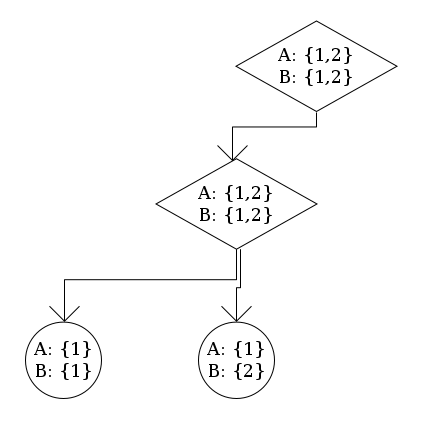
\includegraphics[scale=0.5]{searchExample.png}
  \caption{An example of the backtracking algorithm's attempt to schedule
    travel groups $A$ and $B$ with campsites $1$ and $2$.}
  \label{fig:searchExample}
\end{figure}
%%%%%
% INCLUDE SEARCHEXAMPLE FIGURE
%%%%%

Our solver is optimized to attempt maximal satisfaction of the travelers.
That is, the possible campsites a group may travel to are presented to the
solver in order of ideal travel distance.  While not every group is guaranteed
to always travel their desired distance, the algorithm attempts to satisfy
this ``fuzzy constraint''.  We also calculate the number of encounters
between groups.  After the itineraries are created, each group's campsite
listing is checked to determine how many groups passed and were passed by
this specific group.  By combining the amount of erring from ideal travel distance
and encounters with other groups, we obtain the aforementioned effect on
satisfaction.  This effect is calculated post-solution.
Throughout the course of operation, the solver relies heavily on several
parameters to relax the problem and make solutions more attainable.

\subsection{Usage of High-Level Parameters}
\label{sec:high-params}
% group size
% river length (maybe)
% days in the season
% number of sites
Given some of the information in the prompt and our findings, as discussed
in \textbf{Sections \ref{sec:defs}} and \textbf{\ref{sec:assumptions}}, our program
is designed to adjust its operation depending on various conditions.  The
parameter of greatest variability, number of travel groups, effects how
many groups we generate at the beginning, the load distribution on portions
of the season, and some of the satisfaction scores for other groups. Varying
this value was crucial in analyzing the model, discussed in \textbf{Section
\ref{sec:results}}.

Values that tend to be static include the river length, number of days in
the season, and number of campsites.  While each of these is capable of
drastically effecting the outcome of any given attempt, the values have a
well-defined range (see \textbf{Section \ref{sec:assumptions}}).  The problem
could be generalized beyond these variables such that the CSP solver attempts
to find optimal values for these as well, but this would likely place our
problem into the realm of truly NP-hard problems.


\subsubsection{Tolerance}
Built into the algorithm is a $tolerance$ variable: designed to create a
range for the distance a travel group may cross in a given day.  This variable
is straightforward at the outset but provides several neat nuances for additional
complexity in the solution.  The introduction of a range to the CSP allows
for a larger domain of solutions and, therefore, variability.  In our case,
we desire such flexibility, to account for the real-world implications of
directing human beings.  Tolerance extends within the model as a sort of
aggregate for many of the various instances where we might expect variability
--- such as inclement weather, cancellations, or slow travel groups---,
without having to introduce variability into every aspect.  This may seem
like a stretch of the model's design, but any fuzziness for
any aspect introduces variability into the solutions.  We are satisfied that
tolerance is an opportunistic variable for allowing more groups to be
scheduled and thus for the rafting season to be enjoyed by more individuals.



\section{Predictions and Analysis}
% address all of our graphs
% address the question of how to mix the groups (i.e. oar versus motorized)


\subsection{General Expectations}
\label{sec:expectations}

\subsection{Results}
\label{sec:results}

\subsection{Addressing Carrying Capacity}
\label{sec:capacity}

\subsection{Sensitivity Analysis}
\label{sec:sensitivity}

\section{Conclusions}
\label{sec:conclusions}

\subsection{Advantages to the Approach}
\label{sec:pros}

\subsection{Detractors from the Approach}
\label{sec:cons}

\subsection{Future Extensions}


\subsection{Final Recommendations}
\label{sec:final}




\bibliographystyle{amsplain}
\bibliography{MCM2012.bib}

\end{document}
